\documentclass[letterpaper,11pt]{article}

\usepackage{latexsym}
\usepackage[empty]{fullpage}
\usepackage{titlesec}
\usepackage{marvosym}
\usepackage[usenames,dvipsnames]{color}
\usepackage{verbatim}
\usepackage{enumitem}
\usepackage[hidelinks]{hyperref}
\usepackage{fancyhdr}
\usepackage[english]{babel}
\usepackage{tabularx}
\usepackage{graphicx}
\usepackage{amsmath,amssymb}
\usepackage{booktabs}
\usepackage{multicol}
\usepackage{tikz}
\usetikzlibrary{positioning,calc}
\input{glyphtounicode}

\graphicspath{{portfolio/img/}}

\pagestyle{fancy}
\fancyhf{}
\fancyfoot{}
\renewcommand{\headrulewidth}{0pt}
\renewcommand{\footrulewidth}{0pt}

% Same margins as the resume
\addtolength{\oddsidemargin}{-0.5in}
\addtolength{\evensidemargin}{-0.5in}
\addtolength{\textwidth}{1in}
\addtolength{\topmargin}{-0.8in}
\addtolength{\textheight}{1.35in}

\urlstyle{same}

\raggedbottom
\raggedright
\setlength{\tabcolsep}{0in}
\setlength{\parindent}{0pt}

% Same section format as the resume
\titleformat{\section}{
  \vspace{-4pt}\scshape\raggedright\large
}{}{0em}{}[\color{black}\titlerule \vspace{-5pt}]

\pdfgentounicode=1

% Project heading: title left, links right, rule beneath
\newcommand{\project}[2]{\section{#1 \hfill {\normalfont\small\upshape #2}}}
% Stack line: italic stack, optional bold tag
\newcommand{\stack}[2]{{\small\textit{#1}\if\relax\detokenize{#2}\relax\else\ $|$ \textbf{#2}\fi}\par\vspace{3pt}}
% Two figures side by side with captions; \figh is the maximum figure height
\newlength{\figh}\setlength{\figh}{1.9in}
\newcommand{\figpair}[4]{\par\vspace{5pt}\noindent
  \begin{minipage}[t]{0.47\textwidth}\centering
    \includegraphics[width=\linewidth,height=\figh,keepaspectratio]{#1}\\[2pt]{\footnotesize #2}\end{minipage}\hfill
  \begin{minipage}[t]{0.47\textwidth}\centering
    \includegraphics[width=\linewidth,height=\figh,keepaspectratio]{#3}\\[2pt]{\footnotesize #4}\end{minipage}
  \par\vspace{4pt}}
% Bold subhead above a bullet list; never left alone at the bottom of a page
\newcommand{\subhead}[1]{\par\vspace{4pt}\textbf{#1}\par\nobreak\vspace{-1pt}}
% Run-in bold subhead
\newcommand{\runin}[1]{\par\vspace{3pt}\textbf{#1.}\ }

\newcommand{\resumeItem}[1]{
  \item\small{
    {#1\vspace{-1pt}}
  }
}
\newcommand{\resumeItemListStart}{\begin{itemize}[leftmargin=0.2in]}
\newcommand{\resumeItemListEnd}{\end{itemize}\vspace{-5pt}}

\begin{document}

\begin{center}
    \textbf{\Huge \scshape Portfolio} \\ \vspace{4pt}
    \small Derek Wang $|$ \href{mailto:derek.wang1@uwaterloo.ca}{\underline{derek.wang1@uwaterloo.ca}} $|$
    \href{https://github.com/4ppleSA0CE}{\underline{github.com/4ppleSA0CE}} $|$
    \href{https://www.derekwng.ca/}{\underline{derekwng.ca}}
\end{center}
\vspace{-16pt}

\newcommand{\lnk}[2]{\href{#1}{\underline{#2}}}
% Compact bullet list; \lead is a bold lead-in label
\newenvironment{points}{\begin{itemize}[leftmargin=0.17in, itemsep=1.5pt, topsep=2pt, parsep=0pt, partopsep=0pt, beginpenalty=10000]}{\end{itemize}}
\newcommand{\lead}[1]{\textbf{#1.}\ }
\setlength{\abovedisplayskip}{4pt}\setlength{\belowdisplayskip}{4pt}
\setlength{\abovedisplayshortskip}{2pt}\setlength{\belowdisplayshortskip}{2pt}

%======================= PAGE 1-2: MR. CLEAN =======================
\project{Mr. Clean: LLM-Orchestrated Mobile Manipulation}{\lnk{https://github.com/Karan-Gupta07/Mr.-Clean-Bracketbot-Cleaning-Robot}{GitHub} $|$ \lnk{https://www.youtube.com/watch?v=WjJpOjjXQZs}{Demo} $|$ \lnk{https://devpost.com/software/mr-clean}{Devpost}}
\stack{Python, MuJoCo, PyTorch, Stable-Baselines3, ROS 2, Claude API}{}
{\small\setlength{\figh}{1.3in}
Self-balancing robot with two wheels and two 7-joint arms. Tidies three tables in a simulated MuJoCo room from one typed prompt, with a different controller at each table.

\figpair{mrclean_hero.jpg}{The robot docked at the cube table in MuJoCo}{mrclean_grid.png}{Occupancy grid, footprint inflation (grey) and planned routes (red)}

\subhead{System architecture}
\par\vspace{3pt}\noindent\resizebox{\linewidth}{!}{%
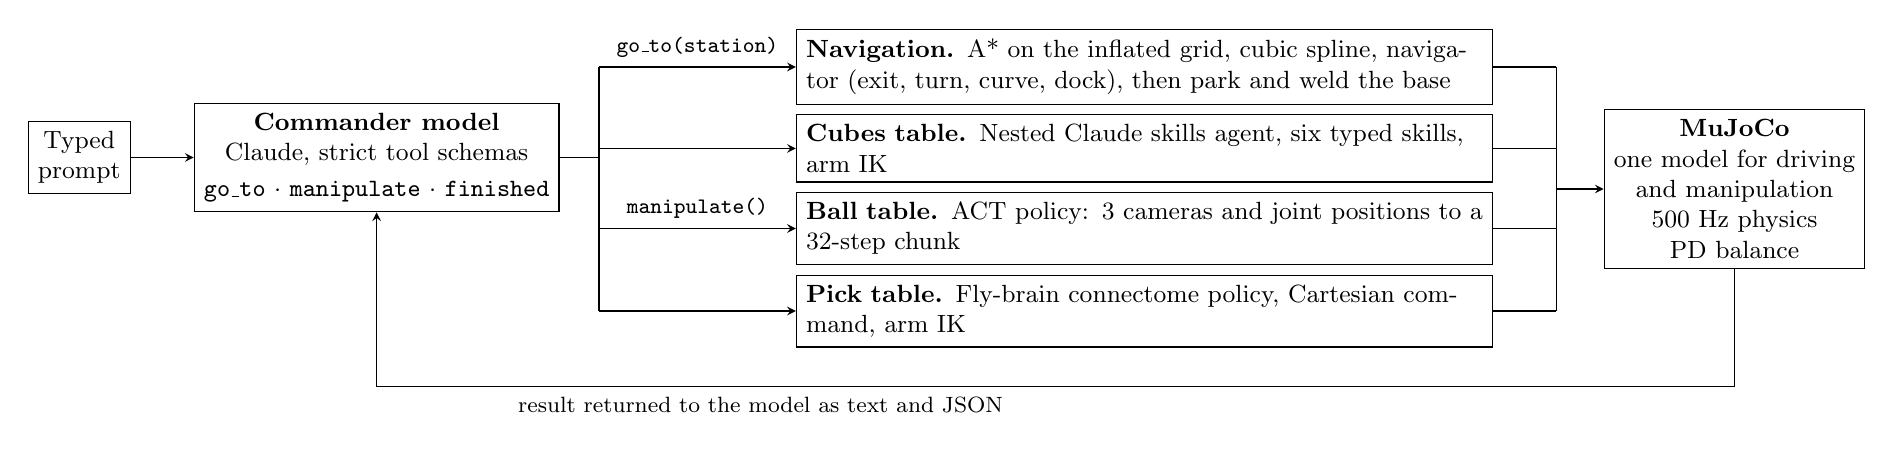
\begin{tikzpicture}[font=\small, >=stealth, box/.style={draw, align=left, inner sep=3.5pt}]
  \node[box, align=center] (prompt) {Typed\\prompt};
  \node[box, align=center, right=8mm of prompt] (cmd) {\textbf{Commander model}\\Claude, strict tool schemas\\[2pt]\texttt{go\_to} $\cdot$ \texttt{manipulate} $\cdot$ \texttt{finished}};
  \node[box, text width=8.6cm, right=30mm of cmd, yshift=11.5mm] (nav) {\textbf{Navigation.} A* on the inflated grid, cubic spline, navigator (exit, turn, curve, dock), then park and weld the base};
  \node[box, text width=8.6cm, below=1.2mm of nav] (cubes) {\textbf{Cubes table.} Nested Claude skills agent, six typed skills, arm IK};
  \node[box, text width=8.6cm, below=1.2mm of cubes] (ball) {\textbf{Ball table.} ACT policy: 3 cameras and joint positions to a 32-step chunk};
  \node[box, text width=8.6cm, below=1.2mm of ball] (pick) {\textbf{Pick table.} Fly-brain connectome policy, Cartesian command, arm IK};
  \coordinate (mid) at ($(nav.east)!0.5!(pick.east)$);
  \node[box, align=center, right=14mm of mid] (sim) {\textbf{MuJoCo}\\one model for driving\\and manipulation\\500 Hz physics\\PD balance};
  % commander to controllers
  \coordinate (busL) at ($(cmd.east)+(5mm,0)$);
  \draw (cmd.east) -- (busL);
  \draw (busL |- nav.west) -- (busL |- pick.west);
  \draw[->] (busL |- nav.west) -- node[above, font=\footnotesize] {\texttt{go\_to(station)}} (nav.west);
  \draw[->] (busL |- cubes.west) -- (cubes.west);
  \draw[->] (busL |- ball.west) -- node[above, font=\footnotesize] {\texttt{manipulate()}} (ball.west);
  \draw[->] (busL |- pick.west) -- (pick.west);
  \draw[->] (prompt.east) -- (cmd.west);
  % controllers to simulation
  \coordinate (busR) at ($(sim.west)+(-6mm,0)$);
  \foreach \n in {nav, cubes, ball, pick} { \draw (\n.east) -- (busR |- \n.east); }
  \draw (busR |- nav.east) -- (busR |- pick.east);
  \draw[->] (busR |- sim.west) -- (sim.west);
  % result back to the commander
  \draw[->] (sim.south) |- ($(pick.south)+(0,-5mm)$) -| node[pos=0.25, below, font=\footnotesize] {result returned to the model as text and JSON} (cmd.south);
\end{tikzpicture}}\par\vspace{2pt}
\begin{points}
  \item \texttt{manipulate()} runs the controller that belongs to the table where the robot is parked; on arrival the base is welded in place and the contact stiffness raised, which gives the arms a fixed platform
  \item No fallback controllers, so a failed station is reported as failed
\end{points}

\subhead{Claude agent controller}
\begin{points}
  \item Two levels, both with strict JSON tool schemas; the nested agent at the cube table has six skills: \texttt{look}, \texttt{pick(object, arm)}, \texttt{place(into)}, \texttt{home}, \texttt{give\_up(object, why)}, \texttt{finished}
  \item Model never receives coordinates; each skill returns a short note, a failure cause from a fixed list, and a symbolic description of the scene
  \item Code selects the arm and retries a grasp up to 8 times inside the skill, so the model decides only the order of the actions
  \item Unknown object names rejected inside the skill with \texttt{object\_not\_found} and the list of valid objects
  \item Limits per run: 2 repeats of an identical failed call, 40 nested steps, 12 top-level steps, no second attempt on an object after \texttt{give\_up}
  \item Live run with \texttt{claude-fable-5-1}: \textbf{4 of 4 cubes sorted in 13 tool calls}
\end{points}

\subhead{Navigation}
\begin{points}
  \item Classical planner for the base, because the robot must not fall and the learned pilot has no obstacle avoidance
  \item Occupancy grid with 5 cm cells, obstacles inflated by 0.26 m for the robot footprint
  \item 8-connected \textbf{A*} without corner cutting, line-of-sight waypoint removal, then a \textbf{clamped cubic spline} through the remaining waypoints
  \item Four route phases (exit, turn, curve, dock); replans at each phase boundary and when the base is more than 15 cm off the path
  \item All \textbf{9 test routes} arrive within 2.4 to 9.6 cm and 1.8 to 4.9 degrees of the goal, with no falls and no furniture contact
\end{points}
}

{\small\setlength{\figh}{1.2in}
\subhead{ACT controller}
\begin{points}
  \item \textbf{Action Chunking Transformer} (Zhao et al., 2023), small enough to train on a laptop
  \item Input: three 128 px camera images (head and two wrists) and 16 joint positions. Output: a chunk of 32 joint commands at 20 Hz, which is 1.6 s of motion
  \item One ImageNet ResNet-18 shared across the cameras, into a transformer with 4 encoder and 4 decoder layers (width 256, 8 heads); 21.9 M parameters
  \item CVAE encoder supplies a 32-dimensional latent $z$ in training, with $z = 0$ at inference. Loss:
  \[ \mathcal{L} = \big\lVert \hat a_{1:32} - a_{1:32} \big\rVert_1 + 10\, D_{\mathrm{KL}}\big( q(z \mid s, a_{1:32}) \,\Vert\, \mathcal{N}(0, I) \big) \]
  \item Overlapping chunks blended with weights $w = \exp(-0.01\,(t - t_0))$; trained on 80 scripted-teacher demonstrations with random ball and crate positions
\end{points}

\figpair{act_frame.jpg}{ACT carrying the ball to the crate}{act_headcam.jpg}{Head camera view, one of three policy inputs}

\subhead{Why ACT has the lowest success rate}
\begin{points}
  \item On new layouts the policy closes on the ball about 4 times in 10 and gets it into the crate \textbf{2 times in 14}; most failures are a ball dropped during the carry or a grasp about 0.5 s too early
  \item \lead{Base pose} Demonstrations recorded with a fixed base. In the full demo the robot parks 2 to 10 cm and up to 5 degrees from that pose, so each camera sees a shifted scene
  \item \lead{Model} Demonstrations used 0.005 armature on the gripper joints. The demo model does not have it, because it causes the cube skills to fail, so it is set only for the ACT episode. Contact pads and solver settings also change when the base parks
  \item \lead{Rendering} A recalculated model constant moved the near plane of each camera from 80 mm to 230 mm and removed the gripper and the ball from the wrist images; 0 of 10 episodes until corrected
  \item \lead{Data} Small data set. The scripted teacher succeeds about 7 times in 10 and drops the ball in one third of its carries, because flat gripper pads do not hold a sphere well
\end{points}

\setlength{\figh}{1.3in}
\figpair{fly_pilot.jpg}{Point-goal pilot driving the base, with live neuron activity}{fly_graph.jpg}{The 512-neuron subgraph at real neuron positions (red excitatory, blue inhibitory)}

\subhead{Fly-brain connectome controller}
\begin{points}
  \item Fruit-fly brain wiring used as the feature extractor of a reinforcement-learning policy
  \item Source: \textbf{FlyWire FAFB v783 connectome} (139,255 neurons, 2.7 M connections). Kept the 64 sensory, 64 descending and 384 central neurons with the most synapses: \textbf{512 neurons and 8,688 edges}, wiring frozen
  \item Synapse counts $c_{ij}$ become signed weights, negative if the presynaptic neuron releases GABA or glutamate, with each row normalised:
  \[ \tilde A_{ij} = s_j\, c_{ij}, \qquad A_{ij} = \tilde A_{ij} \Big/ \max\!\Big(1, \sum\nolimits_k |\tilde A_{ik}|\Big) \]
  \item Observation enters the sensory neurons as an input current $I$ and is propagated for four rounds, with four channels per neuron:
  \[ H^{(t+1)} = \tanh\!\big( 0.35\, H^{(t)} + G \odot \big(A H^{(t)}\big) M^{\top} + I + B \big) \]
  \item Descending-neuron states give a 256-dimensional feature vector for a Stable-Baselines3 policy head
  \item Trained parts: observation encoder, per-neuron gain $G$ and bias $B$, $4 \times 4$ channel mix $M$, and the head. Behaviour cloning from a scripted teacher, then optional PPO
\end{points}
\begin{center}\footnotesize
\begin{tabular}{l@{\hspace{2em}}c@{\hspace{2em}}c}
\toprule
Held-out point goals (20 seeds, 0 falls) & Cloned & Cloned + PPO \\
\midrule
Fly connectome features & 20/20 & 17/20 \\
MLP features & 18/20 & 20/20 \\
\bottomrule
\end{tabular}
\end{center}
\begin{points}
  \item Full connectome needs 1.2 s per forward pass on a CPU against a 50 ms control period, so the graph was reduced to 512 neurons
  \item An MLP gets almost the same results, so no advantage from the fly wiring is shown yet; a shuffled-graph ablation is not yet done
\end{points}
}

%======================= PAGE 3: 7-DOF ARM =======================
\newpage
\project{7-DOF Arm Motion Control}{\lnk{https://github.com/4ppleSA0CE/7-DOF-Arm}{GitHub} $|$ \lnk{https://github.com/4ppleSA0CE/7-DOF-Arm/blob/main/THEORY.md}{Theory}}
\stack{C++17, Eigen, MuJoCo, CMake, React, TypeScript}{No KDL, Pinocchio or MoveIt}
{\small\setlength{\figh}{1.9in}
Motion-control stack for a 7-joint Kinova Gen2 arm in C++17 with Eigen. All kinematics and dynamics code is in the repository, with no robotics library. MuJoCo supplies only the physics simulation and the mesh collision check.

\figpair{arm_dashboard.jpg}{Browser dashboard: drag the target or the obstacle and the arm replans}{arm_dodge.jpg}{Null-space motion: two postures, tool held to 0.2 mm}

\begin{points}
  \item \lead{Redundancy} Controller tracks the tool position, which uses 3 of the 7 degrees of freedom; the other 4 keep the elbow away from obstacles and joint limits while the tool stays on the target
  \item \lead{Rotations and rigid motions} $SO(3)$ and $SE(3)$ with closed-form maps and separate branches for small angles and for angles near $\pi$:
  \[ e^{\hat\omega} = I + \tfrac{\sin\theta}{\theta}\hat\omega + \tfrac{1-\cos\theta}{\theta^2}\hat\omega^2, \qquad
     \mathrm{Ad}_T = \begin{bmatrix} R & 0 \\ \hat p R & R \end{bmatrix} \]
  \item \lead{Forward kinematics} \textbf{Product of exponentials} in body form with home pose $M$ and body screws $B_i$, so the Jacobian and the error twist $\log(T^{-1}T^{*})$ are both in the tool frame:
  \[ T(q) = M \prod_{i=1}^{7} e^{[B_i]\, q_i}, \qquad
     J_{b,i} = \mathrm{Ad}_{\left(e^{[B_{i+1}]q_{i+1}} \cdots\, e^{[B_7]q_7}\right)^{-1}} B_i \]
  \item \lead{Inverse kinematics} \textbf{Damped least squares} on the position Jacobian $J_p$ with a null-space term, $\lambda = 10^{-3}$. Steps stay bounded near singularities, and 26 fixed seeds make each plan reproducible:
  \[ J^{\#} = J_p^{\top}\big(J_p J_p^{\top} + \lambda^2 I\big)^{-1}, \qquad
     \Delta q = J^{\#}(p^{*} - p) + \big(I - J^{\#} J_p\big)\, \dot q_0 \]
  \item \lead{Secondary objectives} $\dot q_0$ sums four terms: face the target, avoid the joint limits, clear the obstacle, clear the scenery. Clearance terms weighted by $w_k = \max(0.3,\, 1 - k/K)$, because at full weight they have no equilibrium when the requested clearance is not possible and the solver does not stop
  \item \lead{Dynamics} \textbf{Recursive Newton-Euler} with twists and wrenches: a forward pass for the link twists $V_i$ and accelerations, a backward pass for the wrenches and joint torques:
  \[ F_i = \mathrm{Ad}^{\top}_{T_{i+1,i}} F_{i+1} + \mathcal{G}_i \dot V_i - \mathrm{ad}^{\top}_{V_i} \mathcal{G}_i V_i, \qquad \tau_i = F_i^{\top} A_i \]
  Gravity $g = \mathrm{RNE}(q, 0, 0)$, Coriolis term $\mathrm{RNE}(q, \dot q, 0) - g$, columns of $M(q)$ from unit accelerations
  \item \lead{Trajectory} Straight line in joint space, $q(s) = q_0 + s\,\Delta q$. Velocity, acceleration and jerk limits of each joint mapped onto $s$ before the move starts, for example $\dot s_{\max} = \min_i v_i / |\Delta q_i|$, so no joint can exceed a limit
  \item \lead{Control} \textbf{Computed torque at 1 kHz} with critically damped gains ($K_p = 196$, $K_d = 28$, $K_i = 30$), friction feedforward, and anti-windup by conditional integration:
  \[ \tau = \big(M(q) + 0.1 I\big)\Big(\ddot q_r + K_d \dot e + K_p e + K_i\!\int\! e\, dt\Big) + C(q, \dot q)\,\dot q + g(q) + \tau_{\mathrm{fric}} \]
  \item \lead{Verification} Forward kinematics and inverse dynamics compared with MuJoCo, Jacobian with finite differences, on 1,000 random configurations each
  \item \lead{Results} 50 motion scenarios with no actuator saturation and no joint reversal. Tip error \textbf{0.2 mm or less on 46 of the 49 reachable targets}; largest 6.7 mm on a sweep point near the base, 6.0 mm on a retarget across the base
  \item \lead{Design choice} IK solved once when the goal or the obstacle moves, never inside the 1 kHz loop. An earlier version solved it each millisecond, needed a 2 cm tolerance, and the arm vibrated
  \item \lead{Limits} Gradient projection moves the arm only along its self-motion manifold, so clearance is not guaranteed in all directions. Simulation only
\end{points}
}

%======================= PAGE 4: STATE ESTIMATION =======================
\newpage
\project{State Estimation and Tracking}{\lnk{https://github.com/4ppleSA0CE/State-Estimation-And-Tracking}{GitHub}}
\stack{C++, Eigen, ROS 2, Python, Docker, KITTI}{0.558 m mean error over 6.6 km $|$ 0.886 MOTA}
{\small\setlength{\figh}{1.7in}
Localization filter and multi-object tracker for a car, in C++ on ROS 2, tested on KITTI. The tracker places detections in the world frame with the pose estimate of the filter, so the localization error propagates into the tracking error.

\figpair{se_hero.png}{Filter estimate against the KITTI reference, drive 0001}{se_gps_dropout.png}{GPS cut for 4 s: track error follows ego error ($r = 0.976$)}

\begin{points}
  \item \lead{Error state} \textbf{15-state error-state Kalman filter} in an ENU map frame with a global attitude error:
  $ \delta x = [\,\delta p,\ \delta v,\ \delta\theta,\ \delta b_a,\ \delta b_g\,] \in \mathbb{R}^{15}$, $q_{\mathrm{true}} = \mathrm{Exp}(\delta\theta) \otimes q $
  \item \lead{Mechanization} Nominal state driven by the 100 Hz IMU, with $a = a_m - b_a$ and $\omega = \omega_m - b_g$:
  \[ p \leftarrow p + v\,\Delta t + \tfrac{1}{2}(Ra + g)\Delta t^2, \qquad v \leftarrow v + (Ra + g)\Delta t, \qquad q \leftarrow q \otimes \mathrm{Exp}(\omega\, \Delta t) \]
  \item \lead{Covariance propagation} $P \leftarrow F_x P F_x^{\top} + Q_d$ with
  {\footnotesize
  \[ F_x = \begin{bmatrix}
  I & I\Delta t & -\tfrac12 [Ra]_\times \Delta t^2 & -\tfrac12 R \Delta t^2 & 0 \\
  0 & I & -[Ra]_\times \Delta t & -R\Delta t & 0 \\
  0 & 0 & I & 0 & -R\Delta t \\
  0 & 0 & 0 & I & 0 \\
  0 & 0 & 0 & 0 & I \end{bmatrix}, \quad
  Q_d = \mathrm{diag}\big(0,\ \sigma_a^2 \Delta t^2,\ \sigma_g^2 \Delta t^2,\ \sigma_{b_a}^2 \Delta t,\ \sigma_{b_g}^2 \Delta t\big) \]}
  \item \lead{GPS update} 10 Hz, lever arm $\ell$, $H = [\,I \ \ 0 \ \ {-[R\ell]_\times} \ \ 0 \ \ 0\,]$. Gain $K = P H^{\top} S^{-1}$ from an LDLT solve, Joseph-form covariance update, then error injection and reset
  \item \lead{Tracker} \textbf{Interacting multiple model} filter for each target over constant velocity, constant acceleration and two constant-turn models at $\pm 0.2$ rad/s. With Markov matrix $\Pi$ ($\Pi_{ii} = 0.97$), innovation $y_j$ and its covariance $S_j$:
  \[ c_j = \sum_i \Pi_{ij}\, \mu_i, \qquad \mu_{i|j} = \frac{\Pi_{ij}\, \mu_i}{c_j}, \qquad \mu_j \leftarrow \frac{\mathcal{N}(y_j;\, 0,\, S_j)\; c_j}{\sum_k \mathcal{N}(y_k;\, 0,\, S_k)\; c_k} \]
  \item \lead{Association} Cost $1 - \mathrm{IoU}_{3D}$ with a Jonker-Volgenant assignment; track confirmed after 3 hits and deleted after 3 consecutive misses
  \item \lead{Coupling} Each detection transformed with the filter pose at the exact detection timestamp, $p_e = \hat R\, p_b + \hat t$
\end{points}
\begin{center}\footnotesize
\begin{tabular}{l@{\hspace{1.2em}}r@{\hspace{1.2em}}r@{\hspace{1.2em}}r@{\hspace{1.2em}}r@{\hspace{2.5em}}l@{\hspace{1.2em}}r@{\hspace{1.2em}}r@{\hspace{1.2em}}r@{\hspace{1.2em}}r}
\toprule
Sequence & s & ATE (m) & GPS only & NEES in band & Sequence & s & ATE (m) & GPS only & NEES in band \\
\midrule
09\_26\_0001 & 11.7 & 0.567 & 1.310 & 94.1\% & 09\_30\_0020 & 113.6 & 0.503 & 1.305 & 94.2\% \\
09\_26\_0009 & 27.6 & 0.449 & 1.288 & 94.3\% & 09\_30\_0033 & 166.0 & 1.013 & 1.293 & 56.4\% \\
09\_26\_0015 & 31.3 & 0.436 & 1.264 & 95.8\% & 10\_03\_0042 & 121.9 & 0.575 & 1.298 & 87.1\% \\
09\_26\_0117 & 36.1 & 0.472 & 1.263 & 94.7\% & 09\_29\_0004 & 35.9 & 0.448 & 1.274 & 95.2\% \\
\midrule
 & & & & & Mean & & 0.558 & 1.287 & \\
\bottomrule
\end{tabular}
\end{center}
\begin{points}
  \item \lead{Localization} \textbf{0.558 m} mean trajectory error over eight KITTI sequences (544 s, 6.6 km), 2.3 times better than the GPS fixes that the filter receives
  \item \lead{Cross-check} Each error value calculated by this code and by \texttt{evo}; the run fails if the two differ by more than $10^{-6}$
  \item \lead{Tracking} \textbf{0.886 MOTA} with 5 identity switches on the 11-sequence KITTI Tracking validation split with ground-truth boxes; 0.66 with raw PointRCNN detections and a score gate
  \item \lead{Coupling test} GPS removed for 4 s: ego error rises to 4.5 m, and track error follows with a correlation of 0.976
  \item \lead{ESKF or UKF} A UKF gives the same error at about 24 times the runtime, so the ESKF is used
  \item \lead{Process noise} A larger gyro process noise corrects the overconfident sequence 0033 (1.01 m to 0.53 m) but breaks the 1 degree attitude target on the tuning drive, so the released configuration is unchanged
  \item \lead{Lower bound} A centred moving average of 11 raw fixes has a lower error than the filter on all eight sequences (0.394 m against 0.532 m). It uses future data, so it is a lower bound for a causal filter
  \item \lead{Limits} GPS fixes synthesised from the OXTS reference; the clutter test fails
\end{points}
}

%======================= PAGE 5 =======================
\newpage
\project{WATonomous: Rover Navigation and Perception}{\lnk{https://github.com/4ppleSA0CE/Autonomous-Vehicle-Control-System}{GitHub}}
\stack{C++, ROS 2, Python, YOLO11s, ONNX Runtime}{mAP50 0.96 on 478 validation images}
{\small\setlength{\figh}{1.15in}
\figpair{wato_foxglove.jpg}{Costmap (purple), planned path (green) and the rover in simulation}{wato_yolo.jpg}{Retrained detector on a test image}
\begin{points}
  \item ROS 2 navigation stack in C++: LiDAR scans fill a 30 m by 30 m costmap (10 cm cells, 0.5 m inflation), and a map-memory node merges the local costmaps into a global grid
  \item \textbf{A*} on the global grid with replanning at 2 Hz; \textbf{Pure Pursuit} path following at 10 Hz
  \item Retrained \textbf{YOLO11s} on 3,916 labelled images from two merged data sets to find an orange hammer, a water bottle and a pickaxe
  \item mAP50 0.96 and mAP50-95 0.87 on 478 validation images after 100 epochs; runs on the rover as a ROS 2 node from an \textbf{ONNX} export
\end{points}
}

\project{Reparo: AI Repair Assistant}{\lnk{https://github.com/Karan-Gupta07/RepairBOT}{GitHub}}
\stack{Python, FastAPI, Swift, Gemini, SerpAPI, Reactiv SDK}{Hack Canada 2026 Winner (\$5,000), Most Complex AI Hack Finalist}
{\small\setlength{\figh}{1.15in}
\figpair{reparo_app.jpg}{A sourced replacement part opened inside the App Clip}{reparo_win.jpg}{1st place in the Reactiv track, Hack Canada 2026}
\begin{points}
  \item One photo of a broken device to a structured repair plan in under 60 s, using component detection and \textbf{Gemini} reasoning on the image
  \item \textbf{FastAPI} service converts the LLM output into typed repair models, so the steps, cost estimates and tools always render in the same format
  \item Parts sourced through SerpAPI, Shopify storefront discovery and the Shopify product APIs into one checkout in a Swift Reactiv App Clip
  \item App Clip opens from a QR code or an NFC tag with no installation
\end{points}
}

\project{Silhouette: Cursor for Fashion}{\lnk{https://github.com/Rababb-P/Silhouette}{GitHub} $|$ \lnk{https://www.youtube.com/watch?v=Msyh6SsYRC4}{Demo}}
\stack{Node.js, Next.js, Express, MongoDB, Gemini, Overshoot SDK}{VC referral to continue as a proof of concept for Merian Brothers}
{\small\setlength{\figh}{1.15in}
\figpair{silhouette_1.jpg}{Live camera with body-part tags for the pieces to change}{silhouette_2.jpg}{Generated outfit with shoppable recommendations}
\begin{points}
  \item User takes a photo with the live camera, selects the part of the outfit to change, and picks a style
  \item \textbf{Overshoot} analyses the photo and \textbf{Gemini} generates the new outfit on the image of the user, with links to real products
  \item Gemini pipelines on a MERN stack run inference, product recommendations and style constraints asynchronously, and return recommendations in under 2 s
\end{points}

\runin{Other work} \lnk{https://github.com/Parsa1ll/floaty}{Floaty}: MCP server with 68 tools for the Float Financial API. \lnk{https://github.com/4ppleSA0CE/Hierarchical-Reasoning-Retrieval}{HRR}: LLM-guided tree search for document retrieval. \lnk{https://github.com/4ppleSA0CE/github-repo-analyzer}{GitHub Repo Analyzer}: PDF reports about a repository for different audiences.
}

\end{document}
